% figures/fig2_ordering.tex -- float wrapper for the held-out ordering figure
% (FIGURE 3 in the rendered PDF; cited as \Cref{fig:ordering} from Sec. 5.2).
% Image produced by figures/fig2_ordering.py, which also writes
% figures/out/fig2_ordering_data.json recording every plotted number and the
% file it came from.
%
% NOTATION.  Every drawn label reads \log q_\theta, the clamped positional-flow
% density (endpoint discrete labels held fixed, positional ODE reversed).  It is
% not the joint generator's conditional density and the caption says which
% quantity it is.  The stored record files keep the column name log_p_theta;
% that is a data-file field name and is never drawn.
%
% PROVENANCE
%   panel (a)  figures/out/scale_primary.json, ["dropref"][arm]["per_seed"]
%              [seed]["primary_93"]["pearson_r"], cross-checked at build time
%              against runs/eval_ours/wide_*/boltz_records.csv (both routes
%              agree to 4 decimals; the generator asserts it).
%   panel (b)  runs/eval_ours/wide_*/boltz_records.csv, pert_id 0 dropped,
%              restricted to the 93 ids in figures/out/primary_endpoint.json.
%   panel (c)  figures/out/retrieval_utility.json, ["primary_93"] blocks.  The
%              file's ["oracle"] key is renamed on load: the quantity is the
%              independent evaluator scoring the eSEN TRAINING TEACHER, i.e. an
%              ensemble-specific teacher-evaluator agreement reference, and that is what
%              the legend says.  Its numeral is not printed in the figure.
%   panel (d)  Gaussian side: the same records as (a).  Fixed-RMSD side: the
%              verified pair (value 0.305, flow matching 0.182, gap +0.124,
%              four seeds per arm) carried as constants in the generator.
%              See the ruling below.
%
% RULINGS HONOURED
%   * PANEL (d) IS DRAWN, AND ITS LIMIT IS DRAWN WITH IT.  No artefact under
%     runs/eval_p3 reproduces the verified fixed-RMSD aggregation -- the __cpu
%     round (40 parents, 4 seeds/arm) gives 0.3028 / 0.1885 and the __gpu60
%     round (120 parents, 4 seeds/arm) 0.3505 / 0.2482 -- so the panel plots the
%     verified ARM MEANS ONLY, prints the seed count, draws no per-seed cloud on
%     that side, and says in the panel that the two families are separate rounds
%     on different parent sets and that the comparison is between the gaps.
%     Splicing another round's per-seed cloud under the verified means would be
%     a cross-round comparison and is not done.
%   * The standardised geometry-level scatter that used to be panel (c) is
%     REMOVED.  Its fitted coefficient was algebraically the panel-(a) arm mean,
%     so it restated a number two other panels already carried, and the
%     fixed-RMSD control answers a claim-threatening confound that no other
%     panel addresses.
%   * The scrambled-energy arm is REMOVED from panel (a): only one of its two
%     shards was scrambled, so it is defective, and cell C of \Cref{fig:grid}
%     supersedes it.  No number that the verified register does not carry is
%     drawn anywhere in this figure.
%   * Every arm with three to five seeds shows its raw seed points -- panels
%     (a), (c) and the Gaussian half of (d).
%   * Every "ceiling" and "oracle" label is gone.  The orange marker in panel
%     (c) is the teacher-evaluator agreement reference, labelled ensemble-specific.
%   * NO INFERENTIAL STATISTIC IS DRAWN.  The reporting standard is descriptive:
%     arm means over independently trained seeds, the standard error over those
%     seeds, every raw seed point, the absolute gain Delta r, the seed counts,
%     and the launched/completed/diverged record.  The Welch t and the exact
%     permutation p are still computed as pipeline guards and are written to
%     figures/out/fig2_ordering_data.json, but no t value, no p-value and no
%     significance label reaches the image or the caption.
%   * Palette semantics are the fixed ones: grey = FM-only baseline,
%     green = value/energy.  Vermilion (force) does not appear -- the
%     gradient-supervision baseline is argued in Sec. 5.3.
%   * WIDTH.  This float places the PDF at \linewidth = 5.50 in and the
%     generator DRAWS at 5.50 in (FULL_W = PLACED_FRACTION * TEXTWIDTH_IN with
%     PLACED_FRACTION = 1.00), so the scale on the page is 1.000 and every
%     in-figure point size is a true page point size, none below 7 pt.  An
%     earlier 0.76 placement of a 5.5 in canvas shrank every size to 76% of
%     what the generator asked for; do not go back to it.  Do not \resizebox
%     this float, and if the placement here ever changes, change
%     PLACED_FRACTION in the generator to match.
\begin{figure}[t]
\begin{center}
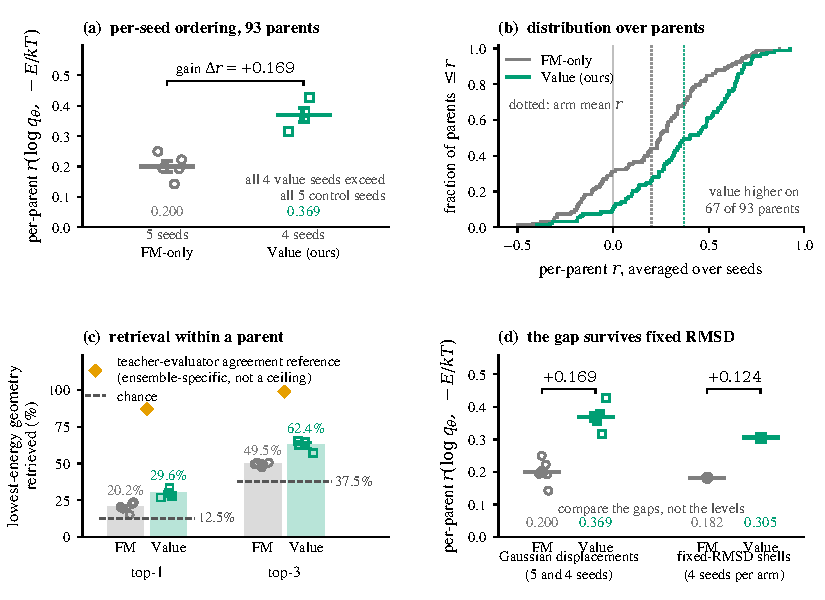
\includegraphics[width=\linewidth]{figures/out/fig2_ordering.pdf}
\end{center}
\caption{Archived readout results; likelihood labels in the plots refer to $\widehat\ell_\theta$, not a validated generator density. \textbf{Energy-value supervision improves local density--energy ordering.}
Population for \textbf{(a)}--\textbf{(c)}: the 93 held-out parents disjoint from the value term's
shard pool, data geometry dropped, up to eight displaced geometries each, scored by GFN2-xTB, an
evaluator independent of the eSEN potential that supplied the training energies. The metric is the
per-parent correlation between the clamped positional-flow density $\log q_\theta$ and $-E/kT$.
\textbf{(a)} Every seed of both arms; rules are arm means, bars their standard error over seeds,
and the gain is $\Delta r = +0.169$ with all four value seeds above all five control seeds. The
value arm is $5/4/1$ launched / completed / diverged, so its mean is conditional on completion.
\textbf{(b)} The shift is spread across the population rather than carried by a few parents.
\textbf{(c)} Ranking a parent's geometries by $\log q_\theta$ retrieves the lowest-energy one more
often; the orange marker is the teacher-evaluator agreement reference (not a ceiling): that
evaluator scoring the training teacher, ensemble-specific and re-measured for any other ensemble.
\textbf{(d)} Holding the within-group displacement magnitude constant to numerical precision leaves
the gap in place, so distance variation is not sufficient to explain the gain; that family is a
separate evaluation round on its own parents with four seeds per arm, and only its arm means are
plotted, so the comparison to make is between the two gaps, not between the two levels. Panel detail in \Cref{app:figdetail}.}
\label{fig:ordering}
\end{figure}
